\documentclass{article}
\usepackage[utf8]{inputenc}
\usepackage{graphicx}
\title{CMSC426HW1 Report}
\author{Yizhan Ao UID: 116022064}
\author{
  Yizhan, Ao\\
  \texttt{josephao@umd.edu}\\
  \texttt{UID:116022064}
}

\date{September 20nd 2021}

\begin{document}

\maketitle

\section{Introduction}

\begin{itemize}
    \item In this report you will be presented with matlab code visualization of geometric representation of Eigenvalues and covariance matrices
    \item The outlier rejection of each datasets with arguing of the optimal choices 
    \item Each rejection technique pros and cons
\end{itemize}

\section{Eigenvalue and Eigenvectors}
\begin{itemize}
    \item Eigenvectors are  vectors that keep their direction after being transformed linearly by any matrix (A). 
    \item Mathematically speaking, $A*v = \lambda*v$ where $\lambda$ lies as a scalar. Also known as Eigenvector.
    \item During $A^T$, eigenvector can find the rotation of a dataset therefore not changing its rotation after the linear transformation 
\end{itemize}

\begin{enumerate}
    \begin{figure1.jpg}
\centerline{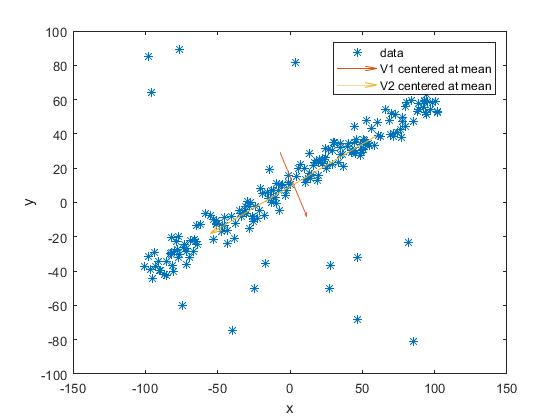
\includegraphics[width=4in, height=3in]{figure1.jpg}}
\end{figure1.jpg}
    
    \item From the dataset 1 we can see the spread and the verticla speed of the data couldnt explain the correlation. Therfore we have to use the covariance of the matrix to explain the magnitude and the direction. The Eigenvectors from the set are having a linear relationship while getting a closer look on the pattern, One arrow is pointing down and one is pointing left down, According to the description of the Problem we have a conclusion that the data is having a low noise. 

     \item The dataset 2 has a moderate noise given a little bit higher coordinates and the linear regression couldn't have an accurate fit. By tuning the noise of the function parameter $\lambda$ we can have a better fit of the model which will need to choose the threshold. RANSAC, also provides a good fit. \begin{figure2.jpg}
{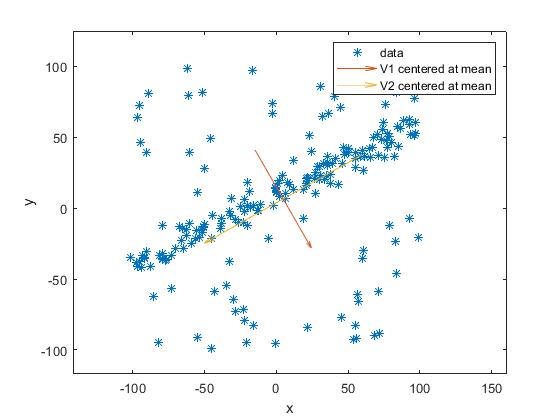
\includegraphics[width=4in, height=3in]{figure2.jpg}}
\end{figure2.jpg}
   
    \item For dataset3 which has a much higher noise and liunear regression is more spread out given coordinates. RANSAC, on the other hand, provides remarkably accurate results when it comes to selecting the appropriate parameters such as inlier threshold, inlier ration, and so on.
    
    \begin{figure3.jpg}
\centerline{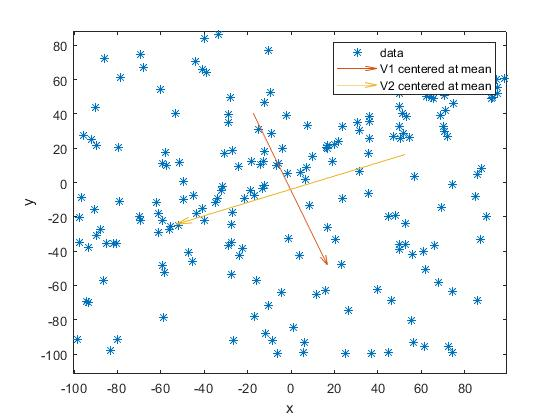
\includegraphics[width=4in, height=3in]{figure3.jpg}}
\end{figure3.jpg}


\end{enumerate}

\section{Optimal Choices}
\begin{itemize}
    \begin{figure4.jpg}
\centerline{\includegraphics[width=4in, height=3in]{figure4.jpg}}
\end{figure4.jpg}
    \item The RANSAC approach is my preferred method since it provides the most visually beautiful fit. However, in terms of algorithm efficiency, I believe the linear method provides a better fit.
    \item From Dataset 2 we have more noise compared to the last dataset. I would say that although  Least Squares lines have the computational efficiency advantage, they do not combat the noise in data 2 well enough
\begin{figure5.jpg}
\centerline{\includegraphics[width=4in, height=3in]{figure5.jpg}}
\end{figure5.jpg} 
    \item For Dataset 3, there are much more noise and more biases. I would say the RANSAC method outperform the Ordinary Least Square in this data set. The Ordinary Least Squares is strongly affected by the noise in the right bottom of the scatter plot. We need to zoom out from the picture to see the whole data points on the picture. Please forgive me for the bad zooming.
 
    \begin{figure6.jpg}
\centerline{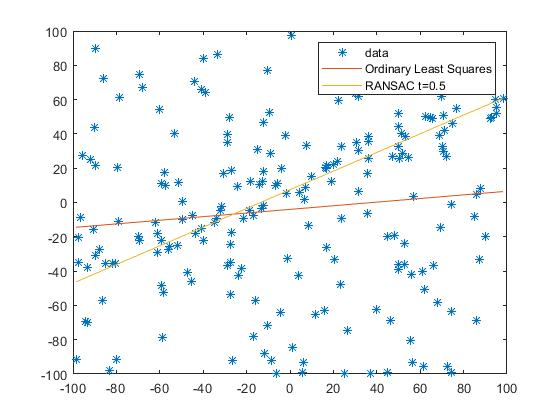
\includegraphics[width=4in, height=3in]{figure6.jpg}}
\end{figure6.jpg}   

\end{itemize}




\section{Limitation of each algorithm:}
    \begin{itemize}
        \item linear Regression works well when the noise is low and the level of boise is low
        \item Regularization has more biance exchanging with variance. Given a dataset which has a low bias but high variance it couldnt do good representation since every possible outcome has a good fitr using least square.  
        \item The RANSAC algorithm is overly reliant on the available computing complexity. Such that, when it comes to determining the problem-specific distance threshold, RANSAC requires more human interaction. Even by human observations, there is no absolute way that which threshold is the most optimal time saver.
    \end{itemize}



\section{References}
\begin{itemize}
    \item https://cmsc426.github.io/math-tutorial/
    \item https://www.visiondummy.com/2014/04/geometric-interpretation-covariance-matrix/
    \item https://en.wikipedia.org/wiki/Random_sample_consensus#:~:text=Random
    \item http://www.cse.yorku.ca/~kosta/CompVis_Notes/ransac.pdf
    \item https://scikit-image.org/docs/dev/auto_examples/transform/plot_ransac.html
    \item https://medium.com/@angel.manzur/got-outliers-ransac-them-f12b6b5f606e
\end{itemize}

\end{document}

